\chapter{Low-Connectivity Reservoirs}\label{ch:low-connectivity}

The choice of ESN metaparameters that best fits a given task is
difficult to identify. In the absence of strong guiding rules, a
practical approach is to treat it as an optimization problem. In this
chapter, I explore using ESNs on the chaotic system forecasting task,
for the Lorenz '63 system, the R{\"{o}}ssler system, and the
double-scroll circuit system described in \cref{ch:systems}. This
exploration is guided by optimization -- by trying to discover the
metaparameters that result in the best averaged NRMSE
$\tilde{\epsilon}$ during forecasting for the given system. This
exploration leads to a surprising discovery, that even ESNs with
simple internal structure perform as well as their more complicated
siblings.

In particular, I am interested in the recurrent connectivity $k$. In
software simulations, such as those described in this thesis, the
connectivity $k$ has only a slight impact on the speed of the
simulation. However, in hardware network implementations, each
connection has an associated cost. For autonomous Boolean networks
implemented on FPGAs, every network connection is built from a long
chain of delay nodes.\cite{canaday2018} These delays often compose the
majority of the resource budget of the hardware network. Although the
results in this chapter are all software simulation, the particular
focus on the $k$ parameter is done with an eye towards hardware
implementations.

Many techniques have been used previously for ESN metaparameter
optimization, such as grid search\cite{rodan2011} and gradient
descent\cite{jaeger2007}. However, both of these approaches have
drawbacks. Grid search quickly becomes intractable when the number of
dimensions grows, and even after fixing the two functional
metaparameters $f$ and $\bm{g}$, there are 5 dimensions
left. Compounding this problem, the ESN construction is a random
process, and so the resulting measured $\tilde{\epsilon}$ for a given
set of metaparameters is a random variable. To get a meaningful
result, each set of metaparameters would need to be tested multiple
times. For even a coarse grid search, with 10 trials and 10 points per
metaparameter, this already means one million trial RCs. Gradient
descent suffers from the randomness of ESN construction as well, for
the same reasons. It is also unsuitable for use with continuous
parameters such as $k$.

The problems with random ESN construction can be mitigated by
modifying the ESN construction method outlined in
\cref{sec:esn-construction} to front-load the random choices. For
example, once the recurrent weight matrix $W_r$ has been constructed,
the parameter $\rho_r$ can be changed without any random process at
all. By cleverly factoring out the random parts of ESN construction,
it becomes possible to use methods like grid search and gradient
descent without the extra step of mulitple random trials. Ultimately,
however, this is optimizing only a single random instantiation of an
ESN, and provides little insight into how the fully random ESN will
perform.

In this chapter, I will be using Bayesian
optimization\cite{yperman2016,maat2018}, as implemented by the
\texttt{skopt} Python package\cite{skopt2018}, to explore which
metaparameters result in the lowest forecasting error
$\tilde{\epsilon}$ for the three example systems. Bayesian
optimization deals well with both noise and integer paramateres like
$k$, is more efficient than grid search,\cite{maat2018} and works well
with minimal tuning.

\section{Bayesian Optimization}

% FIXME cartoon figure for this?
Bayesian optimization is an optimization technique that finds the
minimum of an objective function $h(\bm{x})$ by repeated
evaluation. The process starts with a prior distribution of functions,
representing the algorithm's knowledge of the function $h$. As each
new point $\bm{x}$ is evaluated, the algorithm incorporates this new knowledge
and updates its prior distribution. At the start of the optimization,
points are chosen randomly. This is the exploration phase, where the
Bayesian optimizer is only gathering data to improve it's prior
distribution. After exploration, the optimizer will then evaluate
points $\bm{x}$ with the most expected improvement over the best known minimum
so far.

This algorithm has a number of drawbacks. Primarily, it is
complicated. The above summary only scratches the surface, and already
suggests a number of parameters to the optimization algorithm that can
be tuned, such as the initial prior distribution of functions. This
complication makes it difficult to directly claim that any minimum
found is the true minimum, and so I emphasize that this algorithm is
used here for exploration. I am interested in ESNs that perform well,
and what they have in common, but not in claiming any ESN as the best
performer possible. For this purpose, the unopinionated defaults of
the \texttt{skopt} package suffice.

The complexity of this optimization algorithm also manifests in run
time. After the exploration phase, calculating the next set of trial
parameters $\bm{x}$ involves minimizing an internal function
calculated from the current prior distribution. This can be quite
computationally expensive, and so Bayesian optimization is only
suitable for use when the objective function $h(\bm{x})$ is expensive
enough to justify the extra work to reduce how often it is
evaluated. This makes it a good fit for minimizing prediction error
$\tilde{\epsilon}$ as this involves building, training, and testing
an RC each time.

\begin{table}
  \caption{Range of hyperparameters searched using Bayesian optimization.}
  \begin{tabular}{lrcl}
    Parameter & min & & max \\
    \hline
    $\gamma$ & 7 & -- & 11 \\
    $\sigma$ & 0.1 & -- & 1.0 \\
    $\rho_\text{in}$ & 0.3 & -- & 1.5 \\
    $k$ & 1 & -- & 5 \\
    $\rho_r$ & 0.3 & -- & 1.5 \\
  \end{tabular}%
  \label{tab:bayes-ranges}
\end{table}

In this chapter, the Bayesian algorithm repeatedbly generates a set of
hyperparameters to test within the ranges listen in
\cref{tab:bayes-ranges}. Larger ranges would require a longer
optimization time. I selected these ranges to include values that
existing ESN design heurestics would choose, while also allowing
exploration outside those ranges without a prohibitively long runtime.

During the optimization process, I discovered that the optimizer was
often finding ESNs with $k = 1$ that perform as well as ESNs with a
higher $k$. Such networks have an interesting and simple network
structure, and also suggest other simple structures for comparison.

\section{Structure of Low-Connectivity Reservoirs}

First, networks generated with $k = 1$ often have multiple
disconnected components. For higher $k$, this is still possible but
relatively rare, as $k$ controls the number of opportunities for
components in the network to connect. Disconnected components in the
network essentially act as ESNs operating in parallel. This is an
interesting line of research,\cite{pathak2018} but not one I
investigate further here. In the interest of a more equitable
comparison between $k = 1$ networks and $k > 1$, I discard and
regenerate any networks with more than a single connected component.

\begin{figure}
  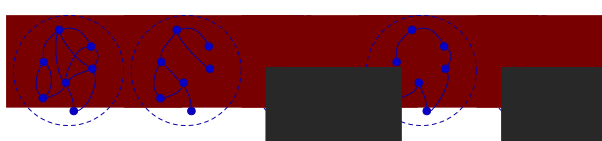
\includegraphics[width=\textwidth]{figures/topology}
  \caption{The five reservoir topologies tested. Only internal
    reservoir connections are pictured. Connections to the reservoir
    computer input, or to the output layer are not shown. (a) A
    general, fixed in-degree network, here pictured with $N=7$ and
    $k=2$. (b) A $k=1$ network with a single connected component. (c)
    A $k=1$ network with the single cycle cut at an arbitrary
    point. (d) A \emph{simple cycle reservoir}. (e) A \emph{delay line
      reservoir}.}%
  \label{fig:topology}
\end{figure}

A $k = 1$ network with only a single connected component must also
contain only a single directed cycle. Starting from any node in the
network and working backwards through the single input connection each
node must have will always lead to a single directed cycle, and it is
not possible for two such cycles to exist in the network unless they
are disconnected from each other. This severely limits how recurrence
can occur inside a $k = 1$ network compared to higher-$k$
networks. Every node in a $k = 1$ network is either part of this core
cycle, or part of a directed tree branching off from this cycle, as
depicted in \cref{fig:topology}~(b).

Inspired by the high performance of this simple structure, I also
investigate $k = 1$ networks when the single cycle is cut at a random
point. This turns the entire network into a tree, as in
\cref{fig:topology}~(c).

Finally, I also investigate reservoir networks that consist entirely
of a cycle or a ring with identical weights with no attached tree
structure, depicted in \cref{fig:topology}~(d), and networks with a
single line of nodes (a cycle that has been cut), in
\cref{fig:topology}~(e). These choices were inspired by the $k = 1$
networks, but have also been researched previously and are known as
\emph{simple cycle reservoirs} and \emph{delay line reservoirs},
respectively.\cite{rodan2011}

In total, there are five network structures I investigate:
\begin{enumerate}[label= (\alph*)]
\item general construction with unrestrained $k$,
\item $k = 1$ with a single cycle,
\item $k = 1$ with a cut cycle,
\item single cycle, or \emph{simple cycle reservoir},
\item single line, or \emph{delay line reservoir}.
\end{enumerate}
Both the $k = 1$ cut cycle networks (c) and line networks (e) are
rescaled to have a fixed $\rho_r$ before the cycle is
cut. However, after the cycle is cut, they both have $\rho_r=0$.

\section{RC Symmetries and their Consequences}

An ESN in autonomous forecast mode, described by \cref{tab:esn}~(b),
has an inversion symmetry about the origin. That is, if $\bm{r}(t)$ is
a solution to this equation, so is $-\bm{r}(t)$. For an output layer
with an identity read-out function $\bm{g}$, this means that if
$\bm{y}(t)$ is a possible output of the trained RC, then so is
$-\bm{y}(t)$. If the underlying system the RC was trained to forecast
also exhibits this symmetry, this is not a problem. In fact, designing
the internal reservoir to match symmetries with the input system can
dramatically improve RC performance\cite{barbosa2021}.

However, if the input system does not have this symmetry, this can be
an issue. If at any time the autonomous forecast strays near $\bm{r} =
0$, the solution can hop over the symmetry to the other side, and
begin producing an output $\bm{y}(t)$ that is flipped through the
origin. This problem is exacerbated if the input signal $\bm{u}(t)$ is
normalized to have mean zero, a common practice.

This problem was identified early, and a common fix\cite{pathak2017,herteux2020}
is to use a non-linear read-out function
\begin{equation}
  g_i(\bm{r}) = \begin{cases}
    r_i & \text{if } i \leq N / 2, \\
    r_i(t)^2 & \text{if } i > N / 2.
  \end{cases}
  \label{eq:esn-break-sym}
\end{equation}
This squares half of the node values before being passed
to the output layer, and breaks the inversion symmetry in the ESN
equation while keeping the number of features accessible to the output
layer the same.

%score: 0.08873905001779689
%score-1: 0.007877037205449461
\begin{figure}
  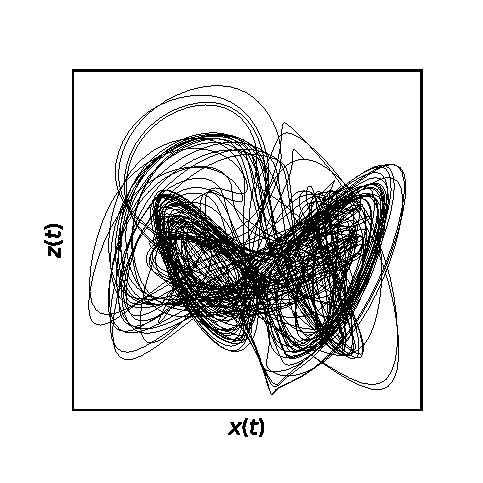
\includegraphics[width=0.6\textwidth]{figures/lorenz-symmetry}
  \caption{The forecasted attractor from an ESN trained on the Lorenz
    '63 system, with identity read-out, in the $x$/$z$ plane. Compare
    against \cref{fig:lorenz}, and note the two deformed images of the
    butterfly attractor on top of each other, with one flipped along
    the $z$ axis.}
  \label{fig:lorenz-symmetry}
\end{figure}

This problem can be difficult to diagnose if the input system has a
partial inversion symmetry. For example, the Lorenz '63 system in
\cref{eq:lorenz} has an $(x, y) \rightarrow (-x, -y)$ symmetry, and so the
complete inversion of the Lorenz attractor looks exactly the same as a
flip along the $z$ axis. This is misleading, as the problem has
nothing to do with the Lorenz $z$ variable specifically, and this
confusion prevented a full understanding of the problem until
recently.\cite{herteux2020} \cref{fig:lorenz-symmetry} provides an
example of the forecasting failure characteristic to the identity
read-out function.

For consistency, I use this \emph{quadratic read-out} for all three
example input systems, even if the inversion symmetry exists in the
input system as it does for the double-scroll circuit.

\section{Training, Forecasting, and Evaluation}

Now that I have identified the five networks structures of interest, I
can use the Bayesian optimization algorithm to identify networks in
each class that perform well on the system forecasting task. I
optimize the metaparameters independently for each of the three
example input systems: Lorenz '63 (\cref{sec:lorenz}), R{\"{o}}ssler
(\cref{sec:rossler}), and the double-scroll circuit
(\cref{sec:dscroll}).

For each input system and for each network structure, the Bayesian
algorithm performs random exploration for 50 iterations, and then
optimization for 50 iterations. At each iteration of the algorithm,
the optimizer constructs a single random instantiation of an ESN with
the chosen metaparameters, trains it, and measures its forecasting
performance with the metric $\tilde{\epsilon}$ defined in
\cref{eq:nrmse-avg}. Since the exploration phase of the optimization
is random, I repeat this entire process 20 times to estimate the
variance in the performance of reservoirs optimized by this method.

To ensure that results are comparable across all three systems, I
normalize their components to have $0$ mean and unit variance. In
addition, I rescale the time axes of all systems so that their maximum
positive Lyapunov exponent matches that of the Lorenz system,
$\lambda_\text{max} = 0.9056$.

To train the ESN, I integrate \cref{eq:esn} with the quadratic readout
in \cref{eq:esn-break-sym}, coupled with the chosen input system, via
the hybrid Runge-Kutta~5(4)\cite{dormand1980} method from $t = 0$ to
$300$. This produces an ESN response $\bm{r}(t)$. I then divide this interval into three ranges:
\begin{itemize}
\item $t = 0$ -- $100$: the warmup period,
\item $t = 100$ -- $200$: the training period,
\item $t = 200$ -- $300$: the testing period.
\end{itemize}
As discussed in \cref{sec:training}, the warmup period is used to
ensure the later times do not depend on the specific initial
conditions of the ESN. I divide the rest into a training period, used
only during training, and a testing period, used later only to
evaluate the ESN performance.

I then determine $W_\text{out}$ via ridge regression, as in
\cref{eq:ridge}, where the sum ranges over the training period. The
ridge parameter $\alpha$ could be included among the metaparameters to
optimize. However, unlike the other metaparameters, modifying $\alpha$
does not require re-integration and can be optimized with simpler
methods. I select an $\alpha$ from among $10^{-5}$ to $10^5$ by
leave-one-out cross-validation. This method also reduces the number of
dimensions the Bayesian algorithm must work with.

To evaluate the performance of the trained ESN, I use it to perform
autonomous forecasting using \cref{tab:esn}~(b). I choose $50$ times
$t_i$ spaced evenly within the testing period. For each $t_i$, I
initialize the reservoir state to $\mathbf{r}(t_i)$, and then
integrate forward with the autonomous equation for one Lyapunov
period, between $t = t_i$ and $t = t_i + 1 / \lambda_\text{max}$. This
produces a reservoir forecast during these times, from which I
calculate an error $\epsilon_{1,i}$ as described in
\cref{eq:nrmse}. Finally, I combine these $50$ errors into a single
$\tilde{\epsilon}$, as in \cref{eq:nrmse-avg}, that represents the
average ability of the ESN to forecast accurately at any point on the
input system attractor.

\begin{figure}
  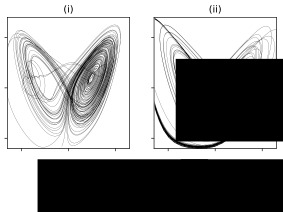
\includegraphics[width=0.6\textwidth]{figures/epsilon-failure}
  \caption{Two examples of reservoir computers that fail to reproduce
    the Lorenz attractor, but produce a low $\epsilon_1$. Compare with
    the true attractor in \cref{fig:lorenz}. Reservoir (i) fails to
    learn the attractor, overemphasizing the right lobe in which $t_1$
    resides. Reservoir (ii) matches the attractor well early on, but
    as the prediction lengthens, it falls into a periodic orbit (thick
    black line). Both (i) and (ii) show a promising low $\epsilon_1$,
    but the averaged $\tilde{\epsilon}$ measure more accurately
    captures their failure to learn the Lorenz attractor.}%
  \label{fig:epsilon-failure}
\end{figure}

Using $\tilde{\epsilon}$ and not simply $\epsilon_1$ is even more
important in an optimization setting, as searching for ESNs with the
lowest $\epsilon_1$ risks producing ESNs that are only good at
forecasts near $t_1$, but otherwise perform poorly in reproducing the
attractor of their input system. It can also waste time, as the
optimization algorithm explores areas of the parameter space it
believes perform well, but actually do not. \Cref{fig:epsilon-failure}
depicts two common ways for an RC to fail to replicate the true Lorenz
attractor, shown in \cref{fig:lorenz}. However, both produce a good
short-term forecast near $t_1$. In particular, reservoir (ii) in
\cref{fig:epsilon-failure} has a lower $\epsilon_1$ than any of
the optimized reservoirs despite its obvious failure to learn the
Lorenz attractor.

\section{Results}
% detailed results for lorenz, violin plots, attractors
% for other systems

\section{Cross-task Performance}
% optimized Lorenz used on double-scroll

\section{Conclusion}
% optimization is useful, and can yield surprising results
% \tilde{\epsilon} is good
% rho_r = 0, k=1 are useful (weird!)
% but: they are rarer. This might be useful
% NARX note: also look forward to next chapter. what unifies these?
% line reservoir is almost just some time delay taps
% can this generalize to many tasks? can it make hardware simpler?
